\documentclass{article}
\usepackage[final]{nips_2017}
\usepackage{graphicx,amsmath,amssymb,booktabs,xcolor}
\usepackage{caption}
\usepackage[colorlinks=true,allcolors=blue]{hyperref}
\captionsetup{font=small,labelfont=bf}

\makeatletter  % neutral preprint footer instead of the NIPS conference notice
\def\@noticestring{Preprint. Work in progress. Companion to ``Paraphrase Bottlenecks.''}
\makeatother

\title{Reading the Router: Plain-Language Profiles of\\
Mixture-of-Experts Specialization}
\author{%
  Steven Hou\\
  Independent Researcher}

\begin{document}
\maketitle

\begin{abstract}
\noindent
A companion paper argued that AI oversight benefits from rendering a model's
opaque internals into plain English---there, by paraphrasing a chain of thought.
Here we apply the same legibility agenda to a different internal: the
\emph{routing} of a Mixture-of-Experts (MoE) model. We extract genuine per-token
expert assignments from OLMoE-1B-7B (16 layers, 64 experts, top-8) on a
category-labeled corpus, quantify how specialized each expert is, and hand each
specialized expert's distinctive tokens to a small trusted model that writes a
one-line, plain-English description of what it does. We find that (i)~most experts
are \emph{balanced} (mean specialization $0.19$), but (ii)~a legible specialized
tail exists ($2.1\%$ of layer-expert units score $>0.5$) and (iii)~\emph{every}
category has a strongly dedicated expert (peak routing propensity $0.88$--$0.99$
versus a $0.125$ uniform baseline). Specialization concentrates in \emph{late
layers}. The plain-language profiles are frequently accurate and human-readable---a
``calculus and trigonometric notation'' expert, a ``Python syntax'' expert, a
``speech verbs and quotation marks'' expert, and shared Romance-language experts.
We argue router-level plain-language profiling is a cheap, model-agnostic
legibility tool, and we are honest about its limits: specialization is modest,
category-defined, correlational, and the descriptions are only as good as the
labeller.\footnote{Code and data: local artifact at
\texttt{\textasciitilde/moe\_legibility/}. Single 7B-MoE, $1{,}541$-token corpus
proof of concept; Section~\ref{sec:lim} states scope.}
\end{abstract}

\section{Introduction}
Mixture-of-Experts (MoE) models replace a dense feed-forward block with many
``experts'' and a router that sends each token to a sparse top-$k$ subset
\citep{shazeer2017moe,fedus2022switch}. This buys parameter count without
proportional compute, and powers strong open models \citep{jiang2024mixtral,
muennighoff2024olmoe}. But the router is opaque: a long-standing question is
\emph{what each expert specializes in}, and answers have been mixed---\citet{jiang2024mixtral}
report little obvious domain structure in Mixtral, while \citet{muennighoff2024olmoe}
find clearer vocabulary and domain specialization in OLMoE.

Our companion paper studied a different opaque internal---a model's chain of
thought---and made it legible for oversight by forcing it through a plain-English
paraphrase. We pursue the \emph{same agenda} for routing: render the expert
structure into plain English so a human can read it. Concretely, we (1)~extract
real per-token routing from OLMoE-1B-7B, (2)~measure each expert's specialization
over a labeled corpus, and (3)~\emph{profile} specialized experts in one plain
sentence each, using a small trusted model as the labeller. The result is a
human-readable map of part of the router.

\paragraph{Contributions.}
(i)~A simple, exact routing-extraction hook and a specialization metric for MoE
experts (Section~\ref{sec:method}).
(ii)~An empirical map of OLMoE specialization: modest on average, concentrated in
late layers, with a strongly-dedicated expert per category
(Section~\ref{sec:results}).
(iii)~\emph{Plain-language expert profiles} generated from genuine routing, with
an honest account of when they are accurate and when they are not
(Section~\ref{sec:profiles}, \ref{sec:lim}).

\section{Method}\label{sec:method}
\paragraph{Model and routing extraction.} We use OLMoE-1B-7B-Instruct
(4-bit)~\citep{muennighoff2024olmoe}: $16$ MoE layers, $64$ experts each, top-$8$
routing, $1.3$B active parameters. We wrap each MoE block's gate to record, for
every token, the indices of its top-$8$ experts at every layer---the exact
selections the model makes, not an approximation.

\paragraph{Corpus and specialization.} We route a corpus of $1{,}541$ tokens
spanning eight categories (Python, math, English, French, Spanish, JSON,
dialogue, Chinese). Let $c_{l,e,k}$ count tokens of category $k$ that select
expert $e$ at layer $l$, and $n_k$ the tokens in category $k$. The routing
\emph{propensity} is $p_{l,e,k}=c_{l,e,k}/n_k$ (expected selections per token; a
uniform router gives $8/64=0.125$). Normalising $p$ over categories to $q$, the
\emph{specialization} of a layer-expert unit is $s_{l,e}=1-H(q_{l,e})/\log 8\in[0,1]$
($0$ = balanced across categories, $1$ = one category).

\paragraph{Plain-language profiling.} For each specialized expert we collect its
\emph{distinctive} tokens---those whose frequency among its selections most
exceeds their corpus frequency (lift)---and give them, with the dominant category,
to a small trusted model (\texttt{llama3.2:3b}) prompted to name the
\emph{token pattern} in $\le 8$ words. This is the legibility step: it converts a
list of token indices into a sentence a person can read.

\section{Results}\label{sec:results}

\paragraph{Specialization is modest but structured.} Mean specialization is
$0.19$: most experts fire across many categories (Fig.~\ref{fig:hist}), echoing
the ``little obvious specialization'' reported for Mixtral. But the distribution
has a legible tail---$2.1\%$ of the $1{,}024$ layer-expert units exceed $0.5$---and
this tail is where plain-language reading pays off. Specialization is not uniform
with depth: it \emph{rises in late layers} (Fig.~\ref{fig:depth}), with the most
specialized experts concentrated in layers 13--15.

\paragraph{Every category has a dedicated expert.} Although the average expert is
balanced, the converse view is striking: for \emph{every} category there exists an
expert it selects with propensity $0.88$--$0.99$---seven to eight times the uniform
baseline (Fig.~\ref{fig:peak}). The category$\times$expert map
(Fig.~\ref{fig:heatmap}) shows the structure directly: bright vertical bands are
specialized experts, French and Spanish light up \emph{the same} experts (shared
Romance-language routing), structured text (Python, math, JSON) shares others, and
English is spread broadly---it is the model's ``default'' register.

\begin{figure}[t]
\centering
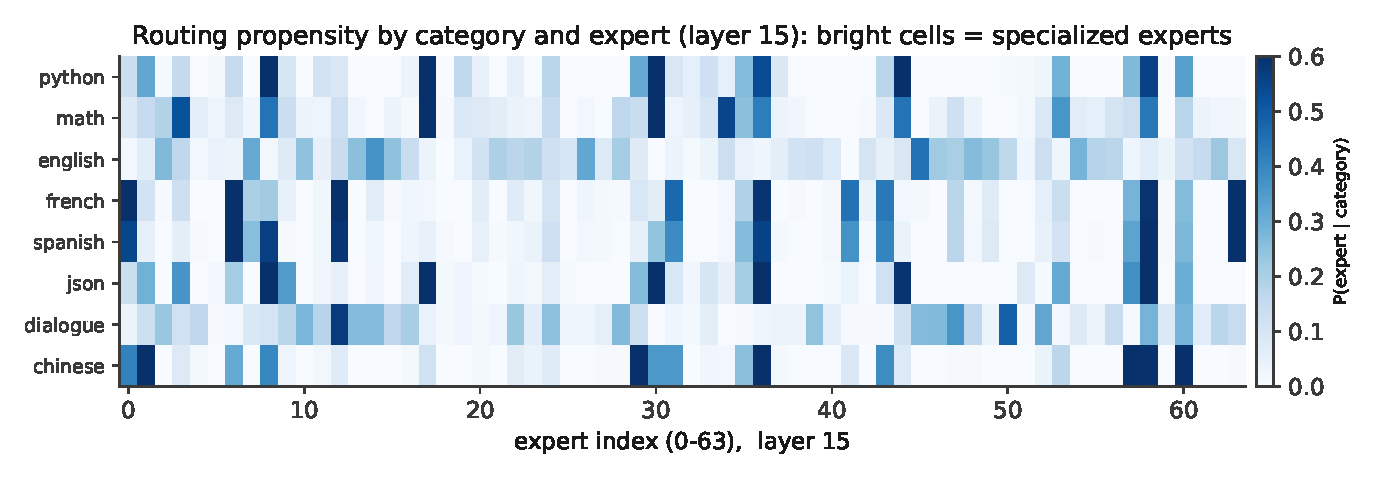
\includegraphics[width=\textwidth]{figures/fig_b_heatmap.pdf}
\caption{Genuine routing propensity $P(\text{expert}\mid\text{category})$ at the
most specialized layer. Bright cells are specialized experts; French/Spanish share
experts, structured text (Python/math/JSON) shares others, English is diffuse.}
\label{fig:heatmap}
\end{figure}

\begin{figure}[t]
\centering
\begin{minipage}{0.32\textwidth}\centering
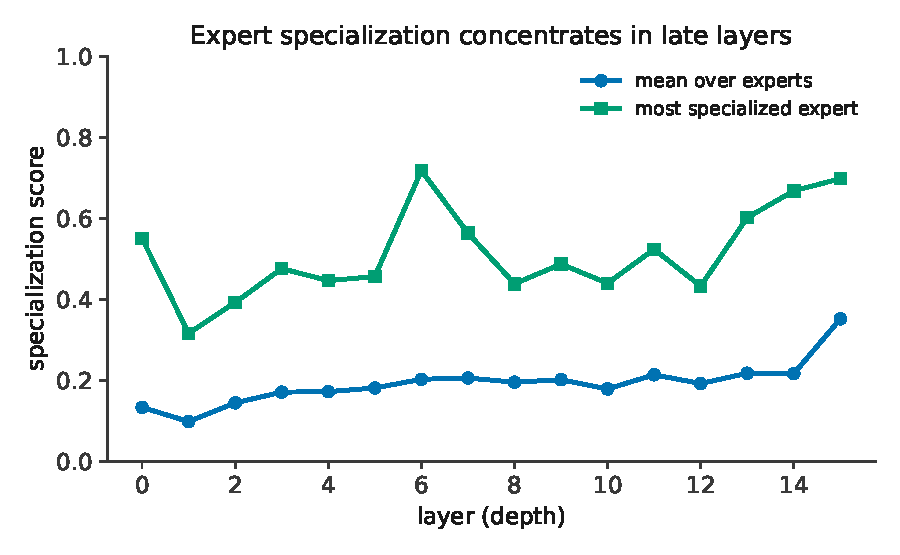
\includegraphics[width=\linewidth]{figures/fig_a_depth.pdf}
\caption{Specialization vs.\ depth.}\label{fig:depth}
\end{minipage}\hfill
\begin{minipage}{0.32\textwidth}\centering
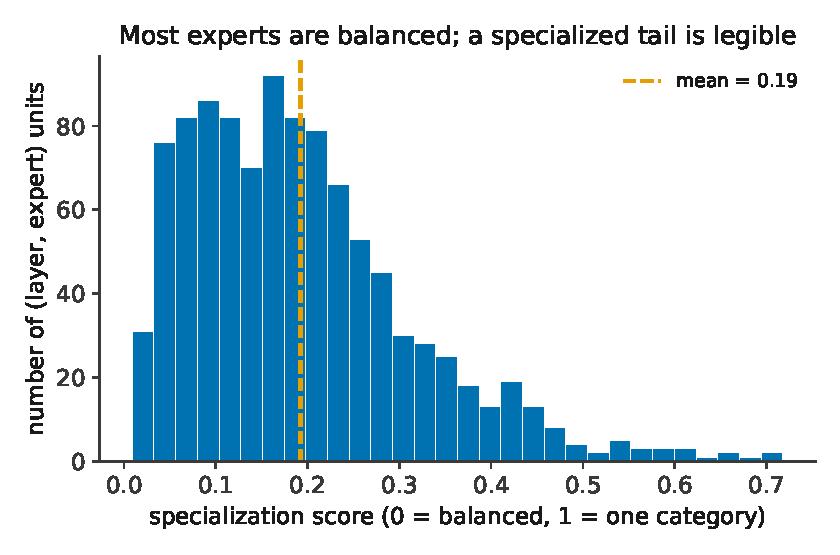
\includegraphics[width=\linewidth]{figures/fig_c_hist.pdf}
\caption{Specialization distribution.}\label{fig:hist}
\end{minipage}\hfill
\begin{minipage}{0.32\textwidth}\centering
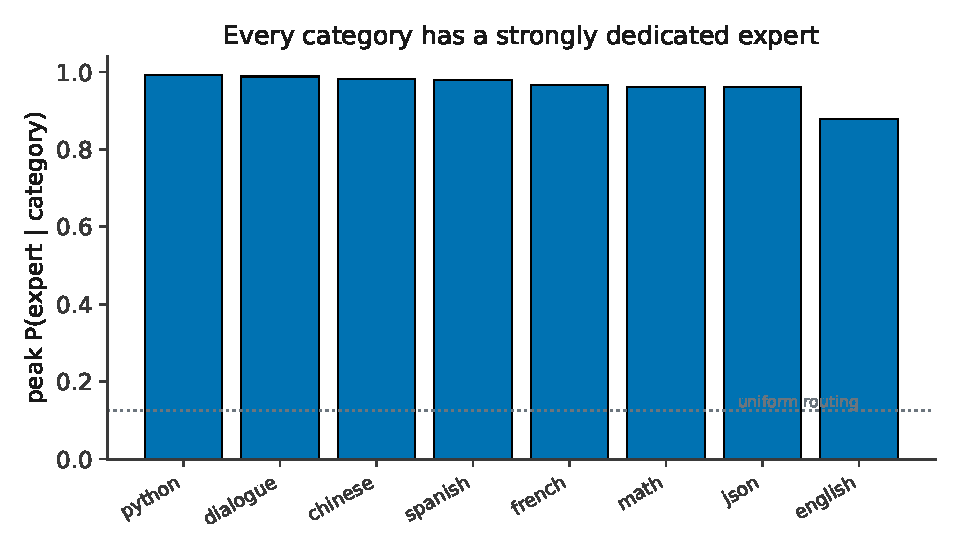
\includegraphics[width=\linewidth]{figures/fig_d_peak.pdf}
\caption{Peak expert per category.}\label{fig:peak}
\end{minipage}
\end{figure}

\subsection{Plain-language expert profiles}\label{sec:profiles}
Table~\ref{tab:profiles} lists profiles generated from genuine routing. Several
are crisp and verifiable against their evidence tokens: a calculus expert
(\texttt{ln, integral, cos, =, /}), a Python-syntax expert
(\texttt{def, return, (, =}), a speech-verb/quotation expert
(\texttt{said, asked, replied}), and a French-function-word expert. These are
exactly the kind of human-readable handles the legibility agenda seeks: one can
look at the router and say, in plain English, what a part of it is for.

\begin{table}[t]
\centering
\caption{Plain-language profiles of specialized OLMoE experts, generated by a
trusted small model from genuine routing. ``L/E'' = layer/expert; $s$ =
specialization.}
\label{tab:profiles}
\small
\begin{tabular}{llll}
\toprule
L/E & $s$ & plain-language profile & evidence tokens \\
\midrule
13/20 & 0.60 & calculus and trigonometric notation & \texttt{ln, integral, equals, cos, *, /} \\
0/52  & 0.55 & Python syntax (def, return, brackets) & \texttt{return, lines, =, (} \\
7/15  & 0.56 & algebraic expressions and symbols & \texttt{equals, of, is} \\
15/39 & 0.69 & speech verbs and quotation marks & \texttt{replied, asked, said} \\
15/26 & 0.61 & French articles and conjunctions & \texttt{la, light, the, and} \\
15/50 & 0.70 & personal pronouns and imperatives & \texttt{I, you, You, me} \\
6/51  & 0.72 & CJK punctuation and dialogue marks & \texttt{,",\ ."} \\
15/21 & 0.56 & negations and interrogatives & \texttt{the, no, a} \\
\bottomrule
\end{tabular}
\end{table}

\section{Discussion}
Read together with the companion paper, a theme emerges: opaque model internals---a
chain of thought, a routing table---can be \emph{partially} rendered into plain
English for human oversight, cheaply and without retraining. For MoE, the win is
real but bounded: the router is not a tidy set of domain modules
(\citealp{jiang2024mixtral}'s caution holds---mean specialization is low), yet it
\emph{does} contain a legible minority of experts that a person can name, and its
coarse structure (late-layer specialization, shared Romance-language experts, a
diffuse English default) is itself interpretable. Plain-language profiling turns
that minority into oversight-ready handles: ``this expert handles arithmetic
notation,'' ``this one handles quoted speech.''

\section{Limitations}\label{sec:lim}
We state scope plainly. (1)~\textbf{Small probe corpus} ($1{,}541$ tokens, eight
hand-chosen categories): specialization scores are category-\emph{defined}---a
different taxonomy would relabel experts, and rare patterns are missed.
(2)~\textbf{Single model}, OLMoE-1B-7B at 4-bit; larger MoEs (Mixtral, DeepSeek)
may differ. (3)~\textbf{Correlational, not causal}: we observe routing, not
expert ablations, so a profile says ``fires on,'' not ``is necessary for.''
(4)~\textbf{Labeller-dependent}: descriptions come from a 3B model and can be wrong
or over-confident (we saw it first mislabel dialogue experts as ``conversational
AI''); the evidence tokens, not the sentence, are the ground truth.
(5)~\textbf{Common-token noise}: pronoun/punctuation experts are harder to name
distinctively than domain experts.

\section{Conclusion}
We read part of an MoE router in plain English. Extracting genuine routing,
measuring specialization, and profiling specialized experts with a trusted small
model yields human-readable descriptions of what experts do---a calculus expert, a
Python expert, a quoted-speech expert---alongside an honest picture of how modest
and structured MoE specialization really is. As with paraphrasing a chain of
thought, the contribution is not that internals become \emph{fully} legible, but
that a useful, oversight-relevant slice of them can be, cheaply.

{\small
\begin{thebibliography}{9}
\itemsep1.5pt
\bibitem[Fedus et al.(2022)]{fedus2022switch} W.~Fedus, B.~Zoph, and N.~Shazeer.
Switch transformers: scaling to trillion parameter models with simple and
efficient sparsity. \emph{JMLR}; \emph{arXiv:2101.03961}, 2022.
\bibitem[Jiang et al.(2024)]{jiang2024mixtral} A.~Jiang et al. Mixtral of experts.
\emph{arXiv:2401.04088}, 2024.
\bibitem[Muennighoff et al.(2024)]{muennighoff2024olmoe} N.~Muennighoff et al.
OLMoE: open mixture-of-experts language models. \emph{arXiv:2409.02060}, 2024.
\bibitem[Shazeer et al.(2017)]{shazeer2017moe} N.~Shazeer et al. Outrageously
large neural networks: the sparsely-gated mixture-of-experts layer.
\emph{ICLR}; \emph{arXiv:1701.06538}, 2017.
\end{thebibliography}
}
\end{document}
